\newpage
\chapter{Methodology}
The initial idea of the thesis is first defined in the following chapter. In the second section, we look at some of the comparable programs that are already on the market. The third section discusses the resulting design considerations necessary for implementing the extension. The fourth section covers the software's design in light of the requirements. The decision to implement the technologies is described in the final section.

\section{Design Concept}
This thesis' original idea is to add an additional feature to Marta's customer-facing platforms. Marta\footnote{\emph{Marta} homepage: \url{https://www.marta.de/}} is currently best described as a marketplace between families requiring 24-hour care and caregivers. 24-hour care can be defined as a period of time spent living in the same household as the individual requiring care. This means that the primary responsibilities of caregivers are basic care and household chores. In addition, they provide assistance to the care recipient's relatives so that they can participate in activities of their choosing. Marta competes with more traditional agencies, where it can take days or even weeks to find a family for a newly registered caregiver or the other way around.

To compete in this rapidly growing industry, Marta would need to improve their product as an expanding startup that has gained a large number of users in recent months. One way in which Marta can provide a superior experience for both caregivers and families is by accelerating the matching process. The caregiver and family inquiry forms are intended to collect as much relevant information as possible for use during the matching phase. The matches are then generated based on the information from the inquiry. To streamline the process, the family is then presented with a number of caregiver profiles that are a good fit for their needs. Filtering capabilities are provided to expedite the search process. This includes the caregiver's earliest start date, German proficiency, disease experience, etc.

To meet the requirements of its users, Marta must implement a continually enhanced, user-friendly filtering capability. An example of a user-friendly filter would be to provide quick filter suggestions that the user can click once to display the desired results, as opposed to allowing users to repeatedly select the same filter manually. To determine which filter suggestions are the most beneficial, it is necessary to identify frequently used filters.

Within this realm of thought, the question of how to enhance the existing filtering functionality for a better user experience arose. An early idea was to create quick filters within the application that would suggest to users which filters they used most frequently. For instance, if a family is seeking a caregiver with level three German language proficiency, the German filter would be activated. Each filter application will be recorded in a relational database. The three most frequently used filters will be displayed as quick filters for all users to activate with a single click. In addition, the user can combine these quick filters to further narrow the search results.

The first issue with this concept was that it collected and stored filter usage data from every user without providing specific information about who used the filter and when. Each family has distinct search criteria. Therefore, the first concept would not be as advantageous to users. Additionally, we must remember that this strategy will only benefit those who actively use the platform. The second concern was that if filter recommendations were personalized for each user, the amount of data maintained would quickly grow to be quite substantial. It would be an inefficient use of storage space, especially as the number of filters and users increases. Not only would we develop quick filters for a single page, but also multiple. And each would necessitate the same quantity of storage space.

The idea was then elaborated upon, and a decision was made. Instead of integrating these quick filters directly into the platform, it would be preferable to create an extension that allows for even more personalized filter suggestions. The aforementioned problems can be resolved by creating an extension. The information that will be saved is user-specific and is stored in the browser of the end user, so the filter suggestions are not affected by the actions of other users. Moreover, search and filter is a common web design technique. It would benefit not only Marta's platform, but also Lacoste, Nike, Adidas, and other e-commerce websites. Moving it to an extension would provide users with the option to install it. And because this is a distinct capability with a different software architecture than Marta's primary platform, a new repository or codebase is created to make it easier to differentiate and manage.

\section{Existing Software}
This section covers the currently available applications or extensions that are similar but do not completely solve the aforementioned problem. There exists a considerable amount of software for manipulating URL parameters but none that provides quick filter suggestions.

\subsection*{Query params}
\emph{Query params}\footnote{\emph{Query params} extension is accessible on: \url{https://chrome.google.com/webstore/detail/query-params/jgacgeahnbmkhdhldifidddbkneahmal}} is an extension for Chrome that gives users the ability to read and write URL query parameters for the tab that is currently active through a graphical user interface. The size of this extension is approximately 85 KB, which is considered to be quite small for an extension of this kind. However, this extension has a purpose that is quite distinct from ours; rather than storing URL parameters, its primary objective is to manage them.

\subsection*{Easy URL Editor}
Another Chrome extension for modifying URL parameters is \emph{Easy URL Editor}\footnote{\emph{Easy URL Editor} extension is accessible on: \url{https://chrome.google.com/webstore/detail/easy-url-editor/kojpdadnbbicdfgfadonheclfpcjpiah}}. The goal of this extension is to make it easier to edit URL parameters for long URLs. This extension allows users to view each URL parameter, add new ones, and delete existing ones. Although they both serve the same purpose, this extension is comparatively larger in size (207 KB) than the previous one.

\subsection*{store-params}
This software, unlike the previous two, is not a browser extension, but rather a vanilla JavaScript library. \emph{Store-params}\footnote{\emph{store-params}'s GitHub repo is accessible on: \url{https://github.com/livechat/store-params}} is lightweight and used for storing URL parameters in cookies, \texttt{localStorage}, or \texttt{sessionStorage} with flexible configuration options. Although there are advantages to using this library, the functionality remains limited. Because this is only a library, it must be integrated with an application to function. It serves the purpose of storing the URL parameters, but not modify them.

\subsection*{ItemsJS}
\emph{ItemsJS}\footnote{\emph{ItemsJS}'s GitHub repo is accessible on: \url{https://github.com/itemsapi/itemsjs}} is another JavaScript library that aims to perform fast searches on JSON datasets. This library differs from the other three mentioned above in that it does not use URLs and instead relies solely on JSON datasets. It is primarily used for data classification of companies, products, publications, documents, and so on. This dependency-free library offers faceted navigation as well as custom full-text search. Since the goal of the thesis is to create a universal solution for every website, this library remains briefly addressed.

Although various software has been released by many developers, this problem is still insufficiently explored. A new approach is therefore needed for the goal of this thesis.

\section{Requirements Elicitation and Analysis}
\label{requirements_analysis}
The extension is used to enhance the user's experience when searching for a desired product or service on an e-commerce website. The plan is to integrate a browser extension into the user's browser that will record the hostname or domain of the visited website's URL along with the corresponding parameters. When sufficient records have been collected, the extension will display a list of domain parameters. These parameters will be separated from path and query parameters. The user is then able to navigate through the path parameters in the same manner as they would a file system. When a path containing parameters is reached, the query parameters and the number of times they are referenced in the URL are displayed. Below the list is an input field and a button; the input field is populated based on the selected parameters and as the user navigates through the list. When the "Navigate" button is clicked, the full-path URL is loaded in a new tab.

The third usability heuristic for user interface design by Jakob Nielsen is user control and freedom. The following statement is made by virtue of this principle, \emph{"Users often choose system functions by mistake and will need a clearly marked emergency exit to leave the unwanted state without having to go through an extended dialogue. Support undo and redo."} \autocite{nielsen1994usability}.

In light of this, the user should be able to return after proceeding. A close button should be included to make it obvious to users how to close the extension. To expand the definition of "user control," users should also be able to customize; they should be able to select which query parameters are saved and which are not.

These prerequisites and considerations result in the following requirements for the extension, which is to be developed within the scope of this thesis. These requirements are classified into functional and non-functional requirements.

\subsection{Functional Requirements}
\label{functional_requirements}
A requirement is called functional if its underlying need is functional, i.e., it relates to information processing objects (data, operations, behavior). In other words, functional requirements are statements of services the system should provide, how the system should react to particular inputs and how the system should behave in particular situations \autocite{sommerville2011software}. The following functional requirements are defined for the extension:

\begin{itemize}
  \item FR-01: User can see how many times each query parameter for each hostname and path name is used
  \item FR-02: User can see a list of paths and parameters based on their history
  \item FR-03: User can assemble a URL query string by selecting a path or a parameter
  \item FR-04: User can navigate to the URL with the assembled query string
  \item FR-05: The extension saves the hostname, path name, and query parameters of the URL
  \item FR-06: The extension stores the URL attributes each time a page is loaded
  \item FR-07: User can define which query parameters should be excluded in the options page
  \item FR-08: User can remove a query parameter count by clicking on the remove icon
  \item FR-09: User can delete all the filters from the options page
  \item FR-10: User can reset the configuration from the options page
\end{itemize}

In addition to functional requirements, non-functional requirements are also defined as follows.

\subsection{Non-Functional Requirements}
A requirement is called non-functional if its underlying need is a non-objective property. In other words, non-functional requirements are constraints on the services or functions offered by the system such as timing constraints, constraints on the development process, standards, etc \autocite{sommerville2011software}. Typically, it applies to the system as a whole, rather than to specific features or services. The following non-functional requirements arise for the extension to be developed:

\begin{itemize}
  \item NFR-01: UI components must be implemented using React.
  \item NFR-02: TypeScript must be used to implement dynamic functions.
  \item NFR-03: Data must be saved on the end-user's Chrome storage.
  \item NFR-04: User's configuration from the options page must be saved on the end-user's Chrome storage.
  \item NFR-05: Both the external components used and the developed component itself must be well documented.
  \item NFR-06: The individual external libraries must be easy to update.
  \item NFR-07: Modularization must be taken into consideration throughout development so that individual modules and/or components can be easily reused, expanded, or changed.
\end{itemize}

While functional requirements are perceived as such by the user, non-functional requirements are implementation details that remain largely hidden from the user.

\section{Software Design}
As the requirements are analyzed, the software's design can now be determined. This section discusses the structure and design patterns of the extension in order to meet the listed requirements. Software development requires a software architecture. It provides a framework for how the software should be constructed, and the decisions made at this stage are essential for the development process moving forward. In light of this, a software architecture diagram is provided.

\autoref{fig:softwareArchitectureDiagram} depicts the components of the software and their interactions with one another. From the software architecture diagram, it is conceivable that there are two major components: Extension core and Chrome APIs. An extension core consists of a user interface and service workers. Content scripts are not displayed, because they are not required for the development of the extension. The extension core would interact with Chrome APIs to persist as well as fetch information on \texttt{chrome.storage} needed for concluding the most used parameters.

The extension's user interface consists of the pop-up and the options page. The pop-up communicates with \texttt{chrome.storage} API to obtain the available filters for the URL's hostname, which is retrieved using \texttt{chrome.tabs} API. Similarly, the options page uses \texttt{chrome.storage} API to get the configuration object rather than the filters. As mentioned in \autoref{service_worker}, a chrome extension has a background script called service worker. The service workers interact with \texttt{chrome.tabs} API to update the filter object on \texttt{chrome.storage} whenever a tab is updated.

\begin{figure}
  \centering
  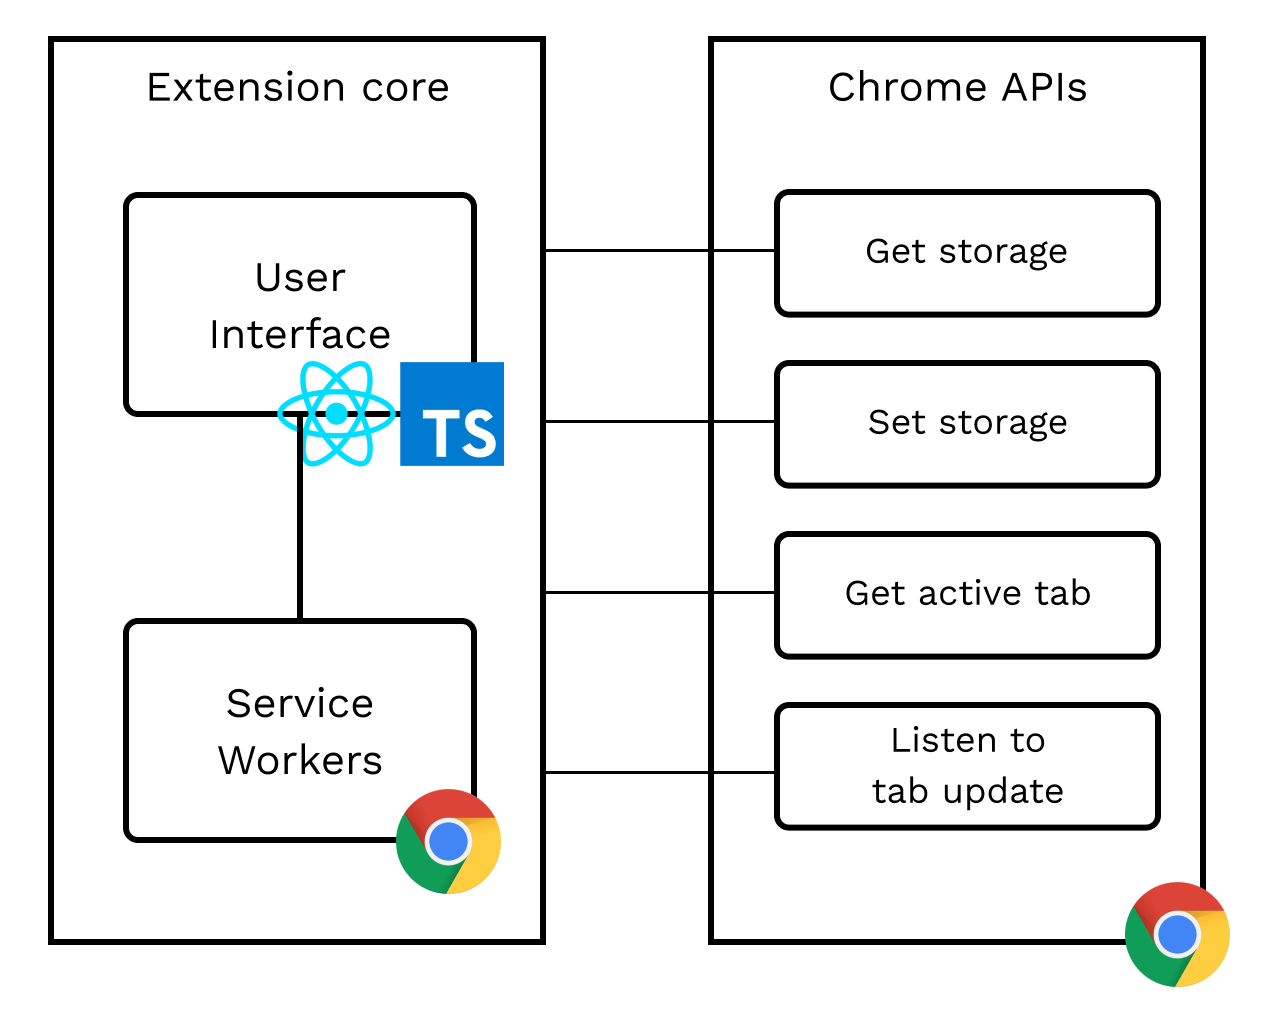
\includegraphics[width=0.7\textwidth]{assets/software_architecture_diagram.png}
  \caption{Software Architecture Diagram}
  \label{fig:softwareArchitectureDiagram}
\end{figure}


\section{Technologies}
\label{technologies_used}
Software architecture does more than just define the software's structure; it can also provide insight into what technologies may be required to build the software. The implementation browser decision will be presented in the next section. The implications of this change on various data storage mechanisms are discussed in the second section.

\subsection{Choice of Implementation Browser}
The selection of a browser was based on a number of factors. The first was the browser's usage rate. This is significant since anyone who doesn't already have the necessary browser will need to download and install it. Drop-outs due to the installation process or being unfamiliar with a new browser can significantly raise the cost of conducting the survey. The ease of use of the API and simplicity of implementation were additional crucial criteria. The extension programming process should ideally only need a basic understanding of the extension API. The capabilities of the API offered by the browser were another factor considered. The extension needs to:

\begin{enumerate}
  \item Store a big amount of data on the client side
  \item Read the URL - so the path and query string can be passed to the extension
  \item Modify the URL - so the most frequently used path and query string can be utilized
  \item Open a full-path URL in a new tab
  \item Access opened tabs
\end{enumerate}

\emph{Internet Explorer}\footnote{\emph{Internet Explorer} is a World Wide Web browser included with Microsoft Windows. Windows 10 deprecated the browser in favor of Microsoft's Edge Browser.} is officially retired and no longer supported as of June 15, 2022, after more than 25 years of facilitating web usage and experience. Consequently, Internet Explorer was removed from the list, leaving Firefox and Chromium-based browsers such as Google Chrome, Microsoft Edge, Opera, and Vivaldi as the only viable options.

Both the Firefox and Chrome extension APIs provide comparable functionality. Firefox's extension technology is, to a large extent, compatible with the extension API utilized by Chromium-based browsers. Most extensions designed for Chromium-based browsers operate in Firefox with very minor modifications. One disadvantage is that Mozilla only supports Manifest V2 and not V3. Since announcing Manifest V3 in 2018, Google has launched Manifest V3 in Chrome, started accepting Manifest V3 extensions in the Chrome Web Store, co-announced joining the W3C WebExtensions Community Group\footnote{The W3C WebExtensions Community Group is formed in collaboration with Apple, Microsoft, and Mozilla.} , and, most recently, laid out a timeline for Manifest V2 deprecation \autocite{alexei2021manifest}. Beginning in January 2022, no new Manifest V2 extensions will be accepted, and Manifest V2 will cease to function in January 2023. Manifest V3 mandates a change to the ecosystem that restricts Manifest V2 extensions and will likely require Manifest V2-based extensions to conform to Manifest V3 in the near future.

\begin{figure}[H]
  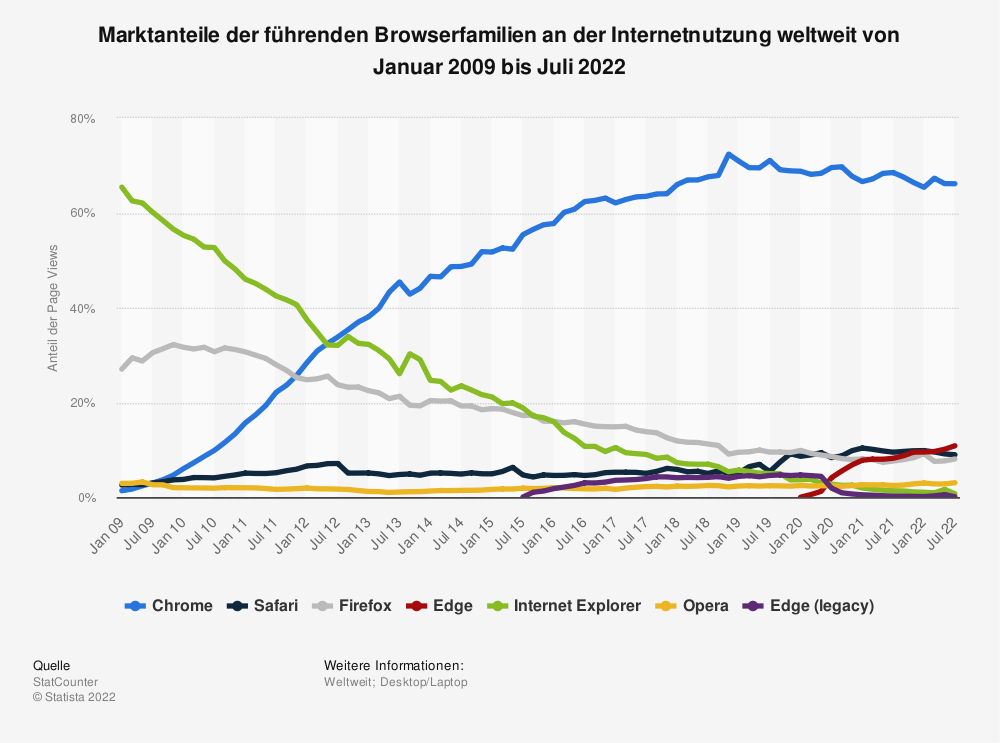
\includegraphics[width=\textwidth]{assets/statistic_id157944_marktanteile-fuehrender-browser-weltweit-bis-juli-2022.png}
  \caption{Market shares of leading browsers worldwide by July 2022}
  \label{fig:browserMarketShareChart}
\end{figure}

Additionally, it was discovered that the Chrome documentation was easy to grasp and was divided up into sections. Over two-thirds of all Internet users worldwide use Chrome as their primary browser (See \autoref{fig:browserMarketShareChart}). As a result, it was decided to develop a Chrome-based browser extension.

\subsection{Data storage}
Data can be stored either on the web server or the web client (the user's computer). Certain data types are better suited for one, while others perform more efficiently on the other. Sensitive and fragile data, for example, should always be stored on the server, whereas static data and user preferences can be stored on the client \autocite{macdonald2013html5}. Currently, most organizations manage various data aspects through various record systems. They have difficulty locating appropriate data stores because they report on each data source separately, resulting in complex data analytics processing. For this project, the types of data that must be stored are specified in \autoref{requirements_analysis}. Client-side storage is used to store and manipulate data in the browser, as no servers are required for this project. The following are instances of data storage and manipulation in the browser:

\begin{itemize}
  \item Maintaining the state of a client-side application, including the current screen, entered data, user preferences, etc.
  \item Utilities with strict privacy requirements that can access local data or files.
  \item Offline progressive web apps (PWAs)
\end{itemize}

\subsection*{Cookies}
HTTP cookies or Cookies were created to keep track of session data on the client side. According to the specification, a Set-Cookie HTTP header with session information was to be sent by the server as part of any response to an HTTP request. Here is an example of the headers in a server's response:

\begin{lstlisting}[language={}, caption={Cookie server response's headers}]
  HTTP/1.1 200 OK
  Content-type: text/html
  Set-Cookie: cookie=any
  Other-header: other-header-value
\end{lstlisting}

The cookie "cookie" with the value "any" is created by this HTTP response. The name and value are both URL-encoded before being sent. Session data is stored in the browser and retransmitted to the server with each request using the Cookie HTTP header, as shown in \autoref{lst:cookieHttpHeader}.

\begin{lstlisting}[language={}, caption={Cookie HTTP header}, label={lst:cookieHttpHeader}]
  GET /index.jsl HTTP/1.1
  Cookie: cookie=any
  Other-header: other-header-value
\end{lstlisting}

This additional data returned to the server can be used to determine the origin of the request. Although cookies provide a simple and well-supported storage mechanism, they have a number of drawbacks. To begin, each cookie is sent back and forth with each HTTP request (via HTTP headers), adding a significant amount of unnecessary overhead. Second, their storage capacity is far insufficient for modern web applications. Third, the same web application that uses cookies cannot run in multiple web browser tabs at the same time. Lastly, the API is somewhat cumbersome \autocite{kessin2011programming, macdonald2013html5}.

\subsection*{Web Storage}
Web storage was first addressed in the Web Applications 1.0 specification of the Web Hypertext Application Technical Working Group (WHAT-WG). Early development of this specification was incorporated into HTML5 before it was separated into its specification. Its purpose is to circumvent some of the limitations imposed by cookies when data is required only on the client side, without the need to constantly send data back to the server. The most recent revision of the Web Storage specification is the second edition. The Web Storage specification's two key goals are to provide a system for storing large amounts of data that survives between sessions and to provide a way to store session data outside of cookies \autocite{frisbie2019professional}.

The second edition of the Web Storage specification defines two types of storage: \texttt{localStorage}, for persistent data, and \texttt{sessionStorage}, for temporary data that is only kept for the duration of a single user session. Until the \texttt{localStorage} object is deleted either by JavaScript or the user by clearing the browser's cache, it will remain accessible. All information stored in \texttt{localStorage} will survive browser restarts, page refreshes, and the closing of all open windows and tabs. However, the \texttt{sessionStorage} object only stores information temporarily, until the browser is closed. This works in a similar way to a session cookie, except that it disappears when the browser is closed. Information saved to \texttt{sessionStorage} is preserved even after the page is refreshed, and depending on the browser's provider, may be accessible even if the browser crashes and is restarted. There are two different ways to store data in the browser that will persist through a page refresh, and both of these APIs are available in modern browsers. LocalStorage and SessionStorage are two types of window properties that have been widely supported by all major browser vendors since 2009.

There are restrictions with Web Storage, just like there are with other client-side data storage options. Some limitations can only be experienced in a certain browser. The client-side data size limit is typically determined per origin (protocol, domain, and port), giving each origin a predetermined amount of storage space. This prohibition is enforced by looking into where the storing page originated from. Aside from that, Web Storage uses synchronous operations, which will cause the main thread to become blocked. In addition, web workers and service workers are unable to access it, and the only type of data that it can store is strings.

\subsection*{IndexedDB}
The Indexed Database API, abbreviated IndexedDB, is a structured data store in the browser. IndexedDB was created as a replacement for the now-deprecated Web SQL Database API. The goal of IndexedDB was to create an API that allowed for the simple storage and retrieval of JavaScript objects while also allowing for querying and searching. IndexedDB is intended to be almost entirely asynchronous. As a result, the majority of operations are performed as requests that will be executed later and produce either a successful or an error result. To determine the outcome of nearly every IndexedDB operation, you must attach \texttt{onerror} and \texttt{onsuccess} event handlers.

It is a key-value browser-based NoSQL (Not Only SQL) data store that operates asynchronously. The NoSQL method of database management is an alternative to the more traditional relational and object-oriented schemas. Instead, NoSQL uses a key/value pair to store information. More than that, the database can store a lot of information, and its API allows for instant access to a practically infinite amount of organized data. But security was not a priority when designing IndexedDB, so it could be seen as insecure.

IndexedDB is a low-level API that necessitates extensive configuration before use, which can be a burden even when storing relatively straightforward information. Instead of relying on promises as most modern APIs do, it uses events instead. Wrappers for the IndexedDB library that provide promises, such as \emph{idb}\footnote{\emph{idb} is a small library that closely resembles the IndexedDB API, albeit with significant usability enhancements. GitHub repository: \url{https://github.com/jakearchibald/idb}}, hide both the powerful features and the complex machinery (such as transactions and schema versioning) that come with using the library.

\subsection*{Chrome Storage API}
Google Chrome provides an API called \texttt{chrome.storage}. This API has been optimized to meet the specific storage needs of extensions \autocite{chrome2021storage}. It allows you to directly synchronize data and persist data across tabs. Asynchronous storage ensures that scripts are not interrupted. As a result, asynchronous saving outperforms synchronous saving in terms of performance. The asynchronous behavior must be considered during implementation. Web Storage or \texttt{localStorage} has a maximum memory limit of 5 MB and does not support tab-spanning storage because the data is only available in the current context. The cross-tab storage and readout are required for the extension's development. Storage-wise, it's very similar to the \texttt{localStorage} API, but there are a few key distinctions:

\begin{itemize}
  \item User data can be synchronized in an automated fashion using \texttt{storage.sync}.
  \item Without requiring a background page, the content scripts of the extension can directly access user data.
  \item Even when using split incognito behavior, a user's extension settings can be saved.
  \item It is faster than the blocking and serial \texttt{localStorage} APIs because it is asynchronous with bulk read and write operations.
  \item Objects can be used to store user data\footnote{The \texttt{localStorage} API stores data in strings}.
  \item It is possible to read the administrator's enterprise policies for the extension using \texttt{storage.managed} with a schema.
\end{itemize}

Using \texttt{chrome.storage} can alleviate the aforementioned limitations with other client-side data storage solutions. Chrome Storage API is well-documented, simple, and takes very little time to set up. Data stored in \texttt{chrome.storage} can be accessed not only from tabs and windows of the same origin. As determined by the JSON stringification of each value and the length of each key, the maximum amount of data that can be stored in local storage is 5MB. However, this value can be ignored if \texttt{unlimitedStorage}\footnote{This permission is only applicable to Web SQL Database and application cache (See issue \url{https://bugs.chromium.org/p/chromium/issues/detail?id=58985}). Additionally, wildcard subdomains such as \url{http://*.example.com} are not supported at this time.} permission is used. Due to the limitations of HTML5 storage in the context of developing a Chrome Extension, the decision is made to use \texttt{chrome.storage}.
